% !TEX program = xelatex % (can also use "lualatex")
%%%%%%%%%%%%%%%%%%%%%%%%%%%%%%%%%%%%%%%%%%%%%%%%%%%%%
%      LaTeX Document Generated by Gemini
%
% IMPORTANT: This document must be compiled with
% XeLaTeX or LuaLaTeX to render CJK characters.
%
% Example compilation command:
% > xelatex your_file_name.tex
%%%%%%%%%%%%%%%%%%%%%%%%%%%%%%%%%%%%%%%%%%%%%%%%%%%%%

\documentclass[11pt]{article}

% --- PACKAGE SETUP ---
\usepackage{geometry}
\geometry{a4paper, margin=1in} % Set margins


\usepackage{xeCJK}     % For Chinese, Japanese, Korean character support

% --- FONT CONFIGURATION ---
% Please ensure you have a CJK font installed.
% Examples: "Noto Serif CJK SC", "Source Han Serif", "MS Mincho"
% Replace "Noto Serif CJK SC" with your chosen font if needed.
\setCJKmainfont{Noto Serif CJK SC}

\usepackage{graphicx}      % For including images
\usepackage{amsmath}       % For advanced math environments
\usepackage{booktabs}      % For professional-quality tables
\usepackage{array}         % For table column formatting
\usepackage{hyperref}      % For clickable links
\usepackage{caption}       % For captions on figures and tables
\usepackage{longtable}     % For tables that span multiple pages
\usepackage[T1]{fontenc}   % For proper font encoding

% --- HYPERLINK SETUP ---
\hypersetup{
    colorlinks=true,
    linkcolor=blue,
    filecolor=magenta,
    urlcolor=cyan,
    pdftitle={The Challenges of Chinese and Japanese Searching},
    pdfauthor={Rauf Aliev},
}

% --- DOCUMENT METADATA ---
\title{The Challenges of Chinese and Japanese Searching}
\author{Rauf Aliev \\ \texttt{r.aliev@gmail.com} \\ TestMySearch.com}
\date{September 2025}

% --- BEGIN DOCUMENT ---
\begin{document}

\maketitle

% --- ABSTRACT ---
\begin{abstract}
The process of tailoring website search functionality for Chinese and Japanese languages presents numerous challenges not commonly encountered with European languages. The way users interact with websites in China and Japan differs significantly, necessitating specialized adaptations for product and content search. The writing systems, which are based wholly or partly on Chinese characters, feature highly irregular orthography and a wide variety of language and character variants. This paper outlines the most significant linguistic quirks and idiosyncrasies that must be considered when implementing a language-aware full-text search. It covers critical aspects such as language detection, character and script variants, word segmentation, normalization, and handling of numerals, synonyms, and homophones. The objective is to provide a comprehensive overview of these issues and demonstrate how they can be addressed using modern information retrieval techniques.
\end{abstract}

\newpage
\tableofcontents
\newpage

% --- ACKNOWLEDGEMENTS ---
\section*{Acknowledgements}
I thank my colleagues for their help in reviewing linguistic details and extending the analysis. I am grateful to \textbf{Timofey Klyubin} for expertise in Japanese and to \textbf{Dmitry Antonov} for valuable feedback, practical tips, and pointers on Chinese.

% --- INTRODUCTION ---
\section{Introduction}
Three languages are traditionally considered together in the context of information retrieval, internationalization, and localization: Chinese, Japanese, and Korean. Their writing systems are based entirely or partly on Chinese characters. This research can be useful for internationalization, localization and information retrieval components and projects. Internationalization is mainly about support for multiple languages and cultures, while localization stands for adaptation of language, content, and design to specific countries, regions, or cultures. Cross-lingual information retrieval deals with documents in one or more different languages, and the techniques for indexing, searching, and retrieving information from large multi-language collections.

From the perspective of information retrieval, Chinese and Japanese present numerous challenges. The major issue is their highly irregular orthography and language variants. In this article, I collected the most important ones we need to take into account when implementing the language-aware full text search as well as how to address them.

% --- LANGUAGE DETECTION ---
\section{Language Detection}
When and where possible, the website should allow the user to specify unambiguously what language is going to be used for entering a search query and presenting the results. Normally, the users enter search queries in the same language as the website’s interface is set to. However, our observations show that the customers use their native language if the website is advertised in their country even if the localized version of the website is not pre-selected, automatically or manually. If the first-level domain is from the local pool (.cn for China or .jp for Japan), the user’s intent of using the native language is even stronger.

To address this case, there are AI and statistical techniques to determine the likely language. The automatic language detection is a very challenging task especially if the analyzed string is short. For example, if it has a mix of Latin and Chinese characters from the Japanese Kanji set, it may indicate that the text is either in Japanese or Chinese, which can be too abstract.

% --- LANGUAGE VARIANTS ---
\section{Language Variants}
\subsection{Dialects}
There are many more dialects in Chinese than Japanese, both full of specificities interesting to us in regard to the topic. Chinese is not a single language; it is a family of spoken languages. China has a lot of dialects, but the most popular are Mandarin (or “Standard Chinese”, over 1 billion speakers) and Cantonese (or Yue, over 100 million speakers). In Japan, there are two major types of the Japanese language: the Tokyo-type (or Eastern) and the Kyoto-Osaka type (or Western). The form that is considered the standard is called “Standard Japanese”. Unlike Traditional and Simplified Chinese, standard Japanese has become prevalent nationwide.

\subsection{Scripts}
\subsubsection{Japanese: Kana and Kanji}
There are two typical Japanese scripts, Kana and Kanji.
\begin{itemize}
    \item \textbf{Kanji} is logographic Chinese scripts, Chinese characters adapted to write Japanese words. There are thousands of kanji in Japanese.
    \item \textbf{Kana} is a collective term for Japanese syllabaries, Hiragana (46 characters) and Katakana (48 characters). They are derived by simplifying Chinese characters selected to represent syllables of Japanese.
\end{itemize}

The same Japanese word can be written in either kana or kanji.

\begin{table}[h!]
    \centering
    \caption{Japanese Script Variants for the word "fox".}
    \begin{tabular}{llll}
    \toprule
    \textbf{English word} & \textbf{Japanese (Kanji)} & \textbf{Japanese (Katakana)} & \textbf{Japanese (Hiragana)} \\
    \midrule
    fox & 狐 & キツネ & きつね \\
    \bottomrule
    \end{tabular}
    \label{tab:fox_variants}
\end{table}

This complexity is also illustrated by the sentence 金の卵を産む鶏 (“A hen that lays golden eggs”). The word ‘egg’ has four variants (卵, 玉子, たまご, タマゴ), ‘chicken’ has three (鶏, にわとり, ニワトリ) and ‘giving birth to’ has two (産む, 生む), which expands to 24 permutations. In many contexts only one option is correct.

Japanese has a large number of loan words or \textit{gairaigo}. The considerable portion of them is derived from English. In written Japanese, gairaigos are usually written in katakana. Many gairaigos have native equivalents in Japanese. Sometimes a Japanese person can use either a native form or its English equivalent written in katakana. This is especially the case of proper names or science terms. If you are not familiar with the native variant, you will probably use a syllabic construct.

\begin{table}[h!]
    \centering
    \caption{Japanese Native Words and English Loan Equivalents.}
    \begin{tabular}{p{0.2\linewidth} p{0.35\linewidth} p{0.35\linewidth}}
    \toprule
    \textbf{English word} & \textbf{Japanese (native word)} & \textbf{Japanese (English loan word)} \\
    \midrule
    door & 扉 /tobira/, 戸 /to/ & ドア /doa/ \\
    mobile phone/cell phone & 携帯 /keitai/, 携帯電話 /keitaidenwa/ & モバイルフォン /mobairufon/, セルラー電話 /serurā denwa/ \\
    \bottomrule
    \end{tabular}
    \label{tab:loan_words}
\end{table}

School kids use hiragana more commonly since they might not have learned the kanji equivalents yet. Additionally, there is Romaji which uses Latin script to represent Japanese.

\subsubsection{Chinese: Traditional and Simplified}
Along with the sheer complexity and size of the character set, Chinese has several related language variants. In Taiwan, Hong Kong, and Macao, Traditional Chinese characters are predominant over the Simplified Chinese variant which is used mainly in Mainland China, Singapore, and Malaysia. Some traditional Chinese characters, or derivatives of them, are also found in Japanese writing. So there is a subset of characters common for different languages. These shared Chinese, Japanese, and Korean characters constitute a set named CJK Unified Ideographs. The CJK part of Unicode defines a total of 87,887 characters, though the characters needed for everyday use is much smaller. For search, queries can be in either traditional or simplified characters or a combination of the two; search results should contain all matching resources, whether traditional or simplified.

Below is a random text to demonstrate the differences between the writing systems. Characters highlighted by yellow marker have different spelling in Simplified (输入简体字点下面繁体字按钮进行在线转换) and Traditional (輸入簡體字點下面繁體字按鈕進行在線轉換) Chinese.

\begin{figure}[h!]
    \centering
    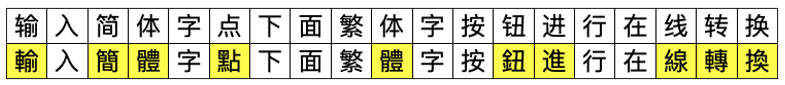
\includegraphics[width=0.8\textwidth]{Screen-Shot-2019-08-19-at-6.39.18-AM.png}
    \caption{Comparison of a sentence in Simplified (top) and Traditional (bottom) Chinese.}
    \label{fig:simplified_traditional}
\end{figure}

% --- CHARACTER VARIANTS ---
\section{Character Variants}
Chinese and Japanese characters don’t use upper or lower cases. They have only a single representation independent of context. The majority of letters are monospaced. There are no additional decorations for the letters as it is in Arabic, for example.

% --- CONVERSION BETWEEN SYSTEMS ---
\section{Conversion Between the Systems}
The conversion is important when either a user or a document uses a mix of Chinese writing systems. For example, given a user query 舊小說 (‘old fiction’ in Traditional Chinese), the results should include matches for 舊小說 (traditional) and 旧小说 (simplified characters for ‘old fiction’). This means that conversion should be done at the query level. The accurate conversion between Simplified Chinese and Traditional Chinese is a deceptively simple but in fact extremely difficult computational task. If your search is used by millions, the system will be much more resource-intensive compared with the setup for European languages.

There are three methods of conversion:
\begin{itemize}
    \item \textbf{Code conversion (codepoint-to-codepoint)}. This method is based on the mapping table and considered the most unreliable because of the numerous one-to-many mappings (in both directions). The rate of conversion failure is unacceptably high.
    \item \textbf{Orthographic conversion}. In this method, the meaningful linguistic units, especially compounds and phrases, are considered. Orthographic mapping tables enable conversion on the word or phrase level rather than the codepoint level. An excellent example is the Chinese word for “computer”.
    \item \textbf{Lexemic conversion}. A more sophisticated, and more challenging, approach to conversion. In this method, the mapping table contains lexemes that are semantically, rather than orthographically, equivalent. This is similar to the difference between \textit{lorry} in British English and \textit{truck} in American English. The complexity of this method lies in lexemic differences between Simplified and Traditional Chinese, especially in technical terms and proper nouns.
\end{itemize}

\begin{table}[h!]
    \centering
    \caption{Examples of Simplified-to-Traditional Chinese Conversion.}
    \begin{tabular}{p{0.25\linewidth} p{0.25\linewidth} p{0.3\linewidth}}
    \toprule
    \textbf{Simplified Chinese} & \textbf{Traditional Chinese} & \textbf{Translation} \\
    \midrule
    干 & 幹 or 乾 or 榦 & (dry, make, surname) \\
    电话 & 電話 & (telephone) \\
    软件 & 軟體 (Taiwan) & (software) \\
    计算机 (“calculating machine”) & 電脳 (“electronic brain”) & (computer) \\
    \bottomrule
    \end{tabular}
    \label{tab:simp_trad_conversion}
\end{table}

In Japanese, the kanji characters may or may not have the same-looking Chinese character.

\begin{table}[h!]
    \centering
    \caption{Character Variation Between Chinese and Japanese.}
    \begin{tabular}{lllll}
    \toprule
    \textbf{Chinese (Simp.)} & \textbf{Chinese (Trad.)} & \textbf{Japanese (Kanji)} & \textbf{Japanese (Kana)} & \textbf{Translation} \\
    \midrule
    两 & 兩 & 両 & & (both) \\
    龟 & 龜 & 亀 & カメ & (tortoise) \\
    \bottomrule
    \end{tabular}
    \label{tab:chinese_japanese_char_var}
\end{table}

It is generally believed that the top priority for Chinese discovery improvements is to equate Traditional characters with Simplified characters. For Japanese, equating Modern (\textit{Shinjitai}) and Traditional (\textit{Kyūjitai}) Kanji is also important—particularly for historical texts, proper nouns, and names—and should not be overlooked in normalization pipelines.

Consider making Simplified Chinese and traditional Chinese inter-searchable. If one searches for 计算机 (computer, Simplified) or 電脳 (computer, Traditional), the results should contain the records with both 计算机 and 電脳. At least measure how often each of these writing systems is used by your customers to make an educated decision on how to make search better.

% --- WORD SEGMENTATION ---
\section{Word Segmentation}
Chinese and Japanese are written in a style that does not delimit word boundaries. Typical Chinese sentences include only Chinese characters, along with a select few punctuation marks and symbols. Typical Japanese sentences include mostly Japanese kana and some adopted Chinese characters that are used in the Japanese writing system. So, how does one decide how to break up the words when there are no separators in between?. As for spaces, they delineate words inconsistently and with variation among writers. Formally, there must always be a space between English words and Chinese words, but in fact this rule is not strict and many neglect it. There is no space between the Arabic numbers and Chinese characters.

There are different approaches for splitting the text into word units. The most common algorithms use dictionaries and, additionally, a set of rules. This topic is still an area of considerable research among the machine learning community. These are not perfect: this segmentation cannot be done unambiguously, but different methods show acceptable results for specific areas. For example, for scientific texts, the dictionary-based methods may show poorer results than statistical or machine-learning based ones.

For example, the word “中华人民共和国” (People’s Republic of China) is seven characters long and has smaller words within: “人民” (people) and “共和国” (republic country). The first two characters,“中华” are usually not be used as a word independently in modern Chinese, though it can be used as a word in ancient Chinese. Digging further, within the word “人民” (people), “人” is a word (human), but “民” (civilian or folk) is not a standalone word. As another example, while the proper segmentation of “中华人民共和国外交部” (Ministry of Foreign Affairs of the PRC) is “中华人民共和国 / 外交 部”, another word, “国外” (overseas), could also be erroneously extracted. Consequently, a search for “国 外” should most likely not match the string “中华人民共和国外交部” but a query for “外 交部” should.

A group of characters might be segmented in different ways resulting in different meanings. The Chinese sentence 我喜欢新西兰花 can be interpreted in two ways, as shown in Table \ref{tab:segmentation_ambiguity}.

\begin{table}[h!]
    \centering
    \caption{Example of Word Segmentation Ambiguity.}
    \begin{tabular}{p{0.3\linewidth} | p{0.15\linewidth} p{0.15\linewidth} p{0.15\linewidth} p{0.15\linewidth}}
    \toprule
    \multicolumn{5}{l}{\textbf{Sentence}: 我喜欢新西兰花} \\
    \midrule
    \textbf{Interpretation 1} & 我 & 喜欢 & 新西兰 & 花 \\
    \textbf{Meaning} & I & like & New Zealand & flower \\
    \midrule
    \textbf{Interpretation 2} & 我 & 喜欢 & 新 & 西兰花 \\
    \textbf{Meaning} & I & like & new & broccoli \\
    \bottomrule
    \end{tabular}
    \label{tab:segmentation_ambiguity}
    \caption*{Note: This ambiguity typically occurs in spoken language. A writer would use the particle 的 to clarify: 我喜欢新的西兰花 for interpretation 1, and 我喜欢新西兰的花 for interpretation 2.}
\end{table}

The challenge is how to extract the meaningful units of knowledge from the text for indexing to return better results at the query phase. There are three approaches:
\begin{itemize}
    \item \textbf{Unigrams}: treat individual Chinese characters as tokens.
    \item \textbf{Bigrams}: treat overlapping groups of two adjacent Chinese characters as tokens.
    \item \textbf{By part of speech or meaningful words}: performs word segmentation and indexes word units as tokens.
\end{itemize}

\begin{table}[h!]
    \centering
    \caption{Tokenization Approaches for “我是中国人” (“I’m a Chinese”).}
    \begin{tabular}{llll}
    \toprule
    & \textbf{Unigrams} & \textbf{Bigrams} & \textbf{Word segmentation} \\
    \midrule
    \textbf{Token 1} & 我 & 我是 & 我 (“I”) \\
    \textbf{Token 2} & 是 & 是中 & 是 (“right”) \\
    \textbf{Token 3} & 中 & 中国 & 中国 (“China”) \\
    \textbf{Token 4} & 国 & 国人 & 人 (“man”) \\
    \textbf{Token 5} & 人 & & \\
    \bottomrule
    \end{tabular}
    \label{tab:tokenization_approaches}
\end{table}

\subsection{Chinese Tokenizers for Apache Solr}
For Chinese, Apache Solr supports various analyzers:
\begin{itemize}
    \item \textbf{Standard Analyzer}: character-based (unigram-like) tokenization; useful as a baseline.
    \item \textbf{ChineseAnalyzer} (deprecated): retained for backward compatibility in older Lucene/Solr versions and not recommended for new deployments.
    \item \textbf{CJKAnalyzer}: indexes bigrams; simple and fast, yielding high recall but low precision as noted above.
    \item \textbf{SmartChineseAnalyzer} (Simplified Chinese only): dictionary + HMM-based; effective for general Simplified Chinese, but limited for Traditional Chinese and often outperformed by modern third-party libraries.
    \item \textbf{HanLPTokenizer} (third-party): modern algorithms (e.g., Viterbi) with strong support for both Simplified and Traditional Chinese; requires separate installation/configuration and typically provides higher accuracy at increased operational complexity.
    \item \textbf{Paoding} (legacy/third-party): an older analyzer that is no longer commonly maintained; generally not recommended for recent Solr versions.
\end{itemize}

\subsubsection{CJKAnalyzer}
This analyzer has a simple bigram tokenizer. It indexes every overlapping two-character sequence without linguistic resources (e.g., “中国人” → “中国”, “国人”). In practice, this yields \textit{high recall} because many queries will find a matching bigram, but \textit{low precision} because unrelated strings can share bigrams. For example, a search for “京都” (Kyoto) can match “東京都” (Tokyo Metropolis) due to the shared bigram “京都”. Likewise, as discussed earlier, one would not want “国外” to match “中华人民共和国外交部”, but bigramming tends to over-match in such cases. A common production practice is to index Chinese simultaneously as words and as overlapping bigrams and combine the methods in a weighted fashion to mitigate noise.
\begin{figure}[h!]
    \centering
    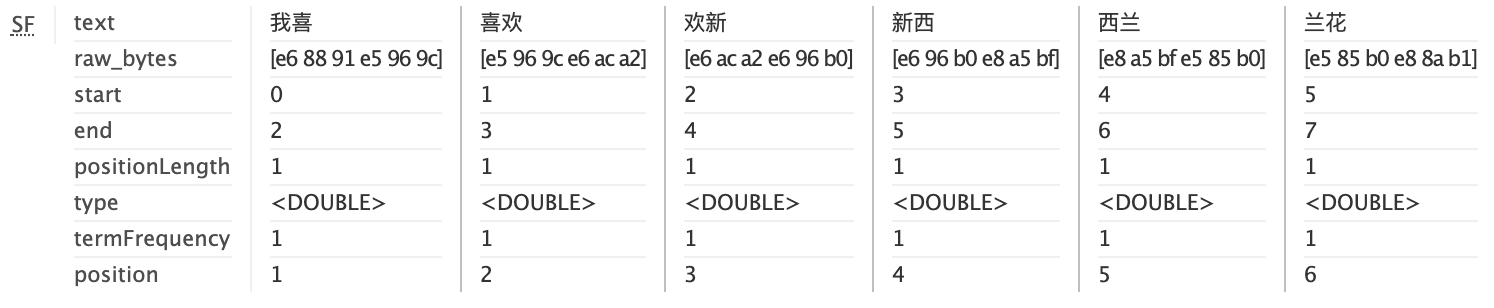
\includegraphics[width=0.7\textwidth]{image2.png}
    \caption{Example of CJKAnalyzer tokenizing a Chinese sentence into bigrams.}
    \label{fig:cjk_analyzer}
\end{figure}

\subsubsection{Smart Chinese Analyzer}
This analyzer uses \textit{HMMChineseTokenizer} which uses probabilistic knowledge to find the optimal word segmentation for Simplified Chinese text. The text is first broken into sentences, then each sentence is segmented into words based on a Hidden Markov Model. It requires a dictionary to provide statistical data, which is included out-of-box from the ICTCLAS1.0 project. SmartChineseAnalyzer creates four terms (I + like + New Zealand (新西兰) + flower) for our example sentence.

It performs well on general Simplified Chinese but does not support Traditional Chinese as effectively as modern external libraries.

\begin{figure}[h!]
    \centering
    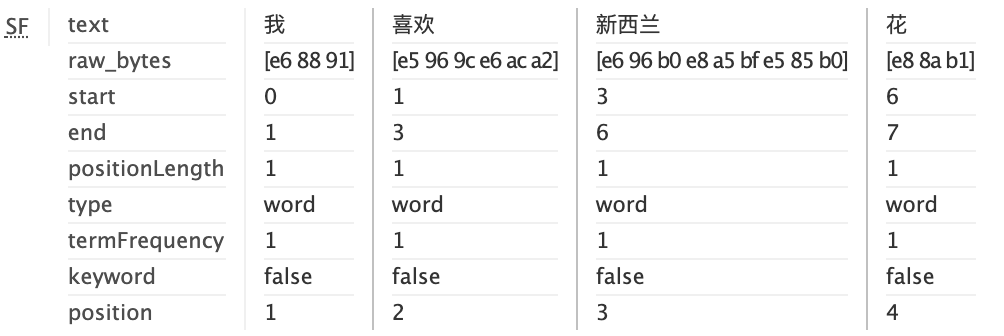
\includegraphics[width=0.7\textwidth]{image3.png}
    \caption{Example of SmartChineseAnalyzer performing word-based segmentation.}
    \label{fig:smart_chinese_analyzer}
\end{figure}

\subsubsection{HanLPTokenizer}
HanLPTokenizer supports multiple algorithms, with the Viterbi algorithm being the default, which offers a good balance of efficiency and effectiveness. Unlike SmartChineseAnalyzer, it supports Traditional Chinese. For our example, HanLPTokenizer creates six terms (I + like + New Zealand (新西兰) + Zealand(西兰) + flower).

Deployments typically require adding HanLP as an external dependency and managing its models, which increases operational complexity relative to built-in analyzers.

\begin{figure}[h!]
    \centering
    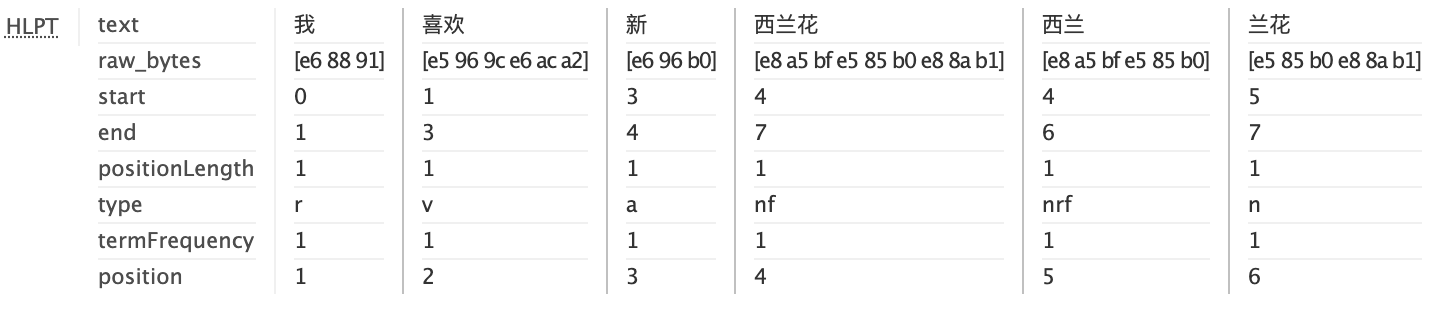
\includegraphics[width=0.7\textwidth]{image4.png}
    \caption{Example of HanLPTokenizer performing word-based segmentation.}
    \label{fig:hanlp_tokenizer}
\end{figure}

\subsection{Domain-Specific Dictionaries and Ongoing Maintenance}
A critical determinant of segmentation quality is the dictionary itself. General-purpose lexicons perform poorly on specialized corpora such as e-commerce product catalogs, biomedical texts, or legal documents. Production systems should plan for:\\
(1) \textit{Domain customization}: seed dictionaries with brand names, SKUs, technical terms, and common compounds;\\
(2) \textit{Feedback loops}: mine query and click logs to identify unknown terms and mis-segmentations;\\
(3) \textit{Versioning and evaluation}: maintain curated releases of dictionaries with regression tests to prevent quality drift.\\
These practices usually yield larger gains than swapping tokenizers alone, and they are essential regardless of the analyzer chosen.

\subsection{Japanese Tokenizers for Apache Solr}
For Japanese, Solr provides:
\begin{itemize}
    \item \textbf{CJKAnalyzer}: indexes bigrams, same as for Chinese.
    \item \textbf{JapaneseTokenizer (Kuromoji)}: splits the text into word units using morphological analysis, and annotates each term with part-of-speech, base form (lemma), reading, and pronunciation.
\end{itemize}

\subsubsection{JapaneseTokenizer (Kuromoji)}
This morphological tokenizer, also known as the Kuromoji Japanese Morphological Analyzer, uses a rolling Viterbi search to find the least cost segmentation (path) of the incoming characters. For our test query “私は日本人です” (“I’m Japanese”), it returns four terms (“I + particle + Japanese + am).

\begin{figure}[h!]
    \centering
    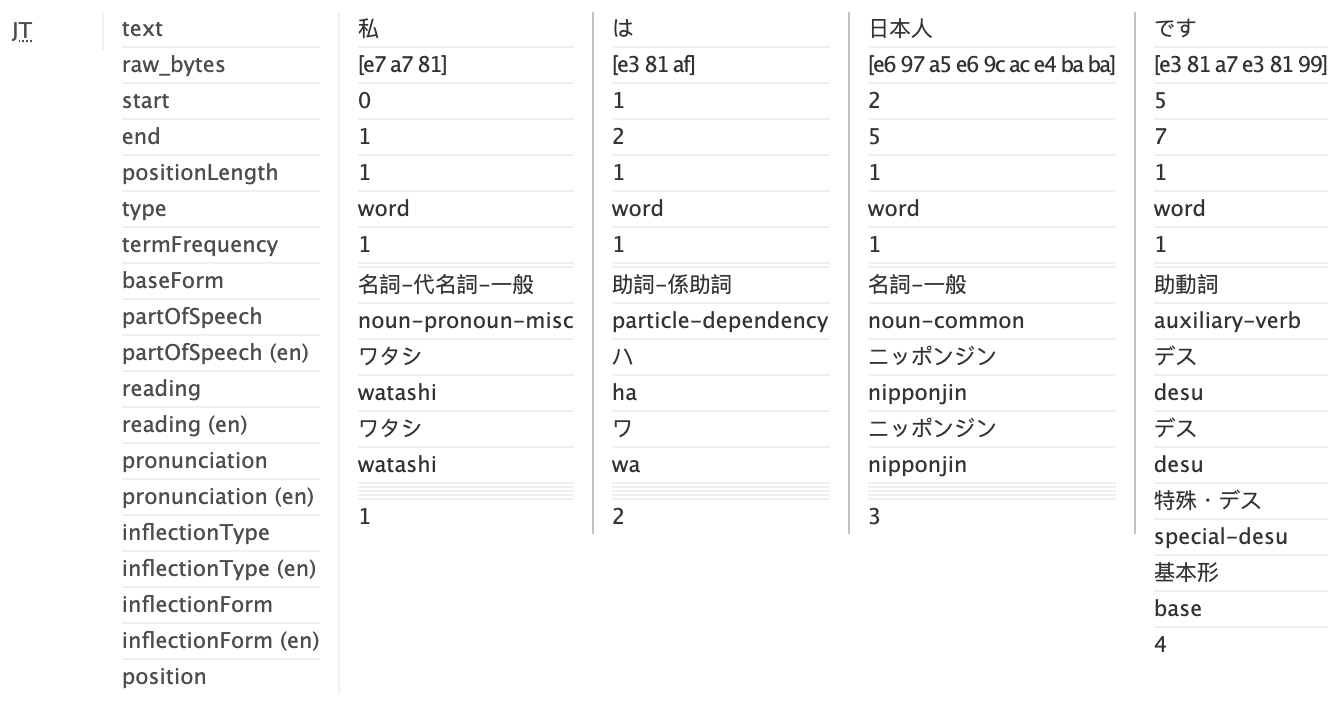
\includegraphics[width=0.7\textwidth]{image5.png}
    \caption{Kuromoji tokenizing “私は日本人です”.}
    \label{fig:kuromoji_example1}
\end{figure}

For a more complex sentence like “韓国に住んでいていい人に聞いた” (I asked a good person, who lives in South Korea), the tokenizer produces a more granular output, but the key point is that the base forms of core words are preserved, maintaining the meaning. Additional tokens like particles can be removed by a stop-words filter.

\begin{figure}[h!]
    \centering
    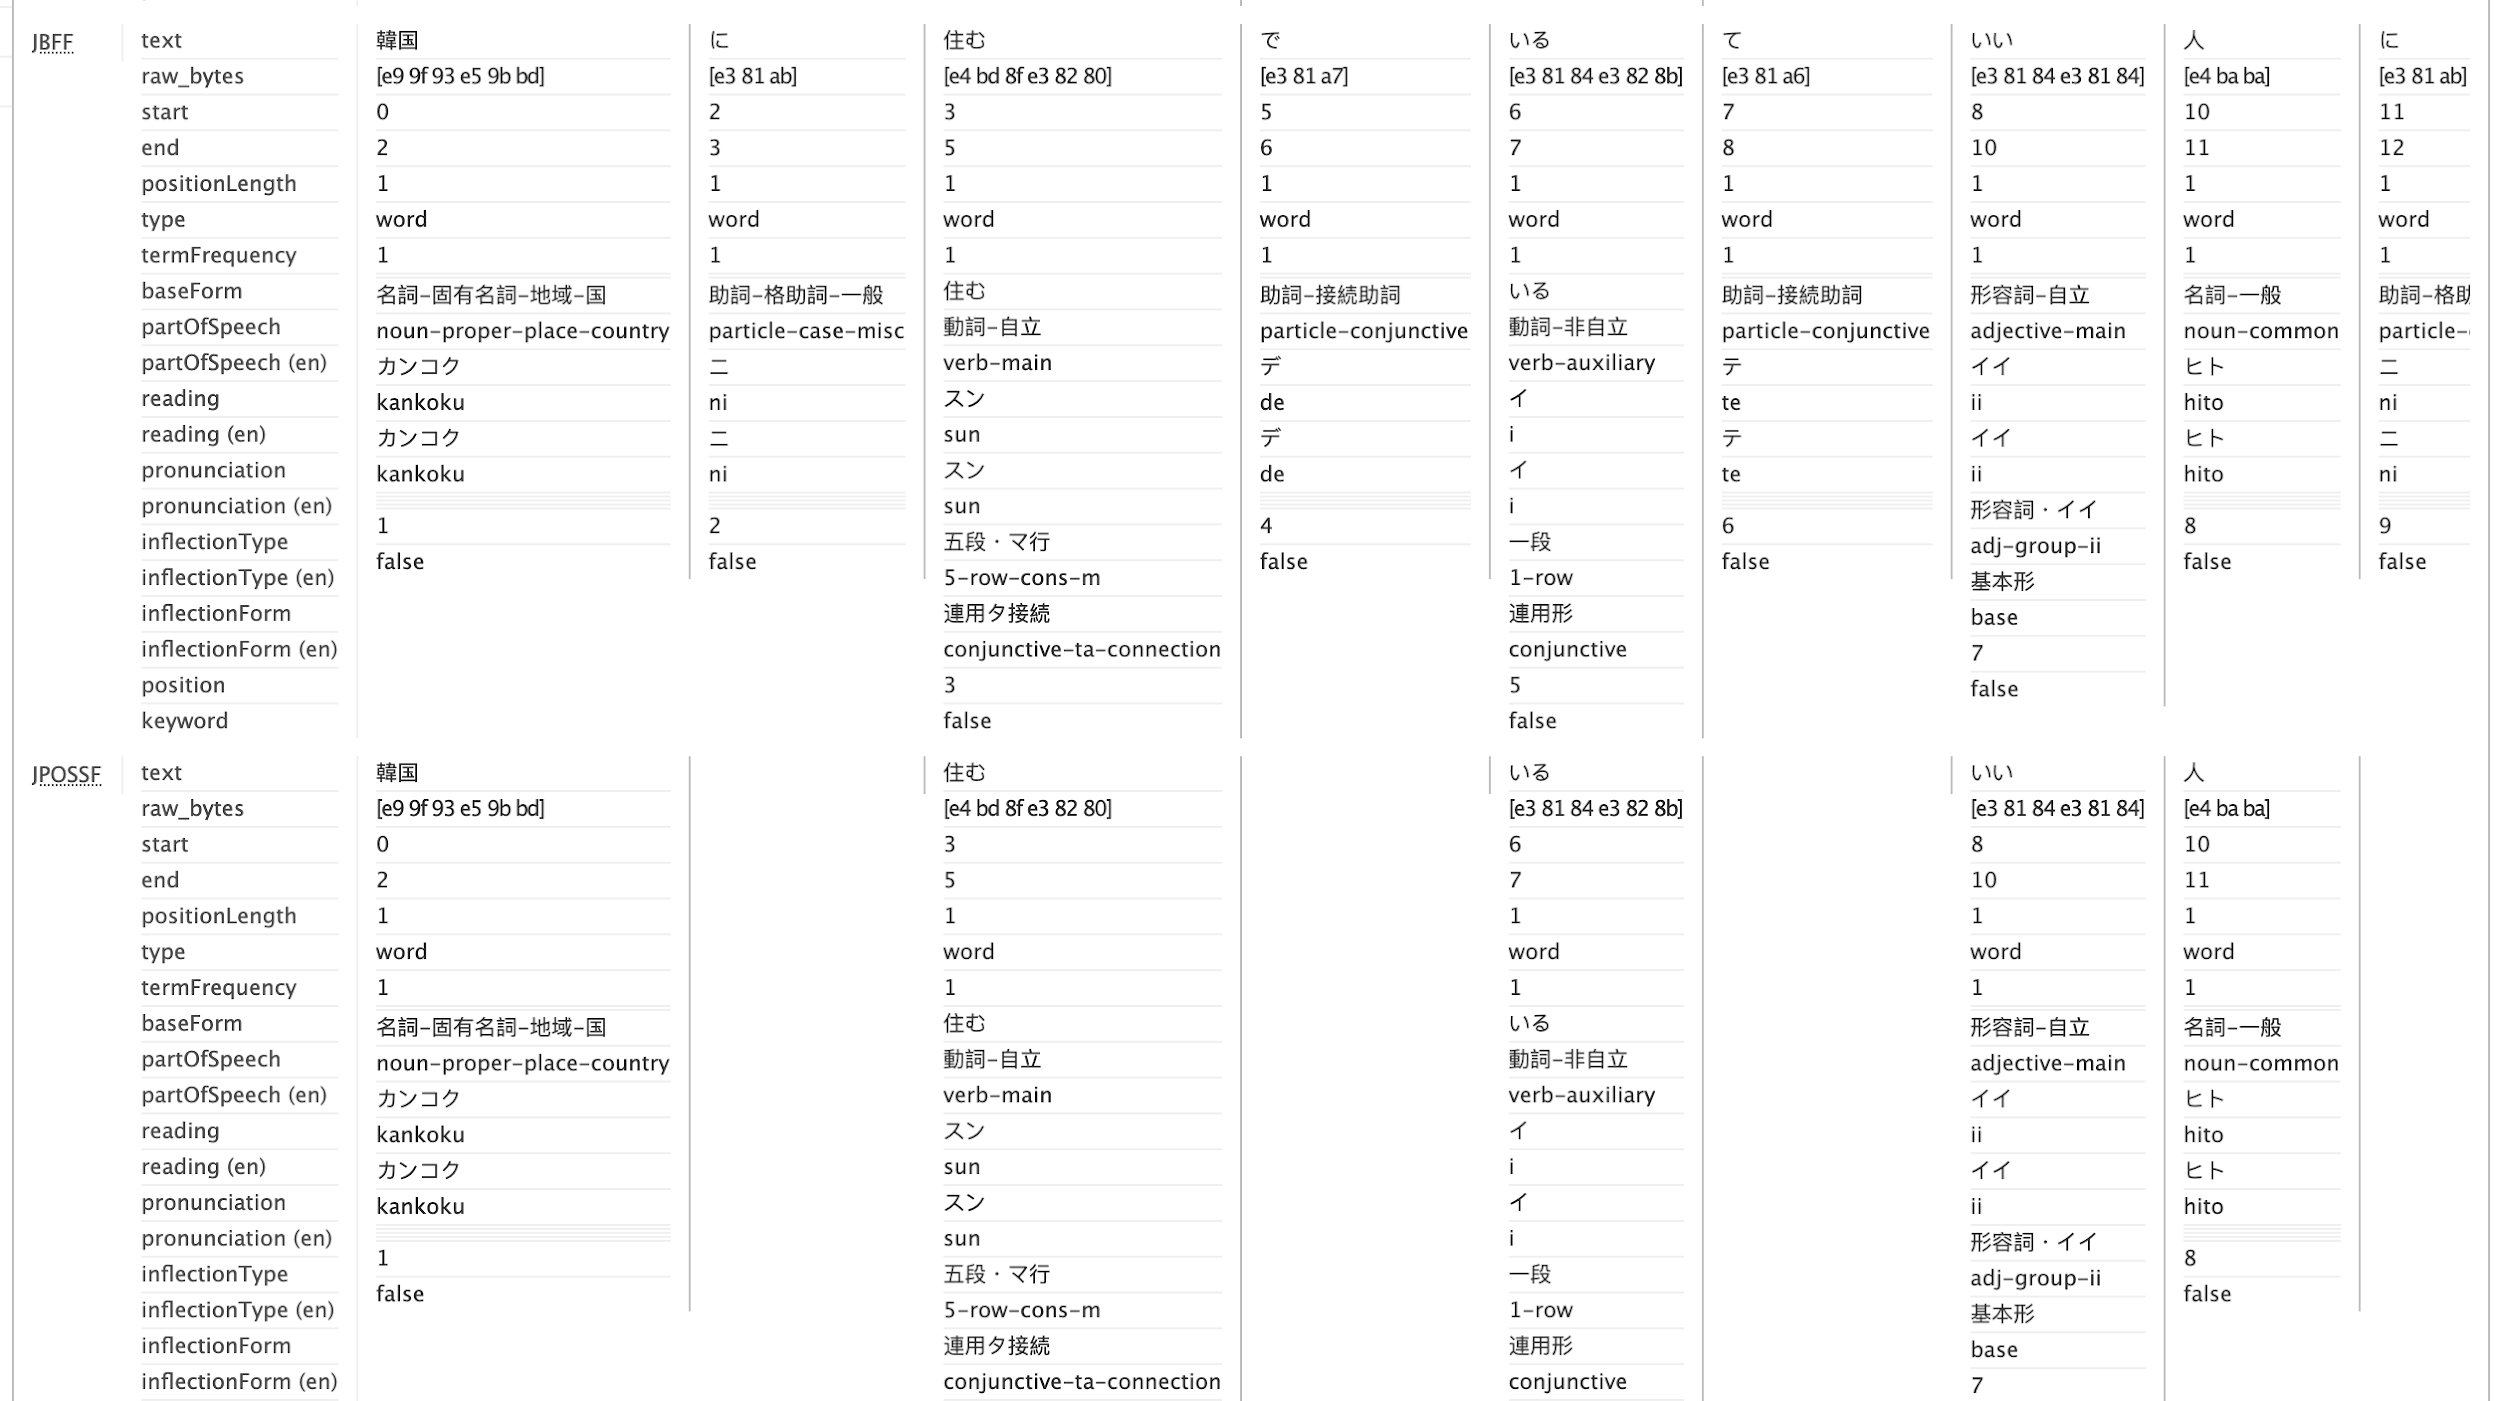
\includegraphics[width=0.9\textwidth]{image6.png}
    \caption{Kuromoji tokenizing a more complex Japanese sentence.}
    \label{fig:kuromoji_example2}
\end{figure}

The tokenizer also supports different modes (\textit{normal}, \textit{search}, and \textit{extended}) to handle compound nouns and provide additional segmentation useful for search. For example, `search` mode can split compounds like 関西国際空港 (Kansai International Airport) to allow a search for 空港 (airport) to match. It might be good to use search mode for indexing and normal mode for queries to increase precision.

% --- WORD NORMALIZATION ---
\section{Word Normalization}
Word normalization refers to the process that maps a word to some canonical form. For example, in English the canonical form for “are”, “is”, and “being” is “be”. This normalization, performed at both index and query time, improves the accuracy of search results. Solr uses two approaches: stemming (reducing a word to its root) and lemmatization (identifying the dictionary form based on context).

\subsection{Solr Filters for Chinese and Japanese}
\subsubsection{Japanese Iteration Marks}
For stemming in Japanese, Solr provides \textit{JapaneseIterationMarkCharFilter} which normalizes horizontal iteration marks (々, odoriji) to their expanded form. These marks are used to represent a duplicated character in the same morpheme, like 人々 (hitobito, "people"), which is normalized to 人人. This is distinct from cases like 日日 (hinichi, "number of days"), where the character is duplicated because it represents different morphemes.

\subsubsection{Half-Width/Full-Width Filter}
By convention, 1/2 Em wide characters are called “half-width”; the others are called correspondingly “full-width” characters. \textit{CJKWidthFilter} folds full-width ASCII variants into the equivalent basic Latin characters (“IjI” -> “IjI”) and half-width Katakana variants into the equivalent standard Japanese kana (カ -> カ).

\subsubsection{Japanese Base Form Filter}
\textit{JapaneseBaseFormFilter} reduces inflected Japanese verbs and adjectives to their base/dictionary forms. For example, for the phrase “それをください。” (That one, please.), ください (kudasai) is converted to its base form, くださる (kudasaru).

\begin{figure}[h!]
    \centering
    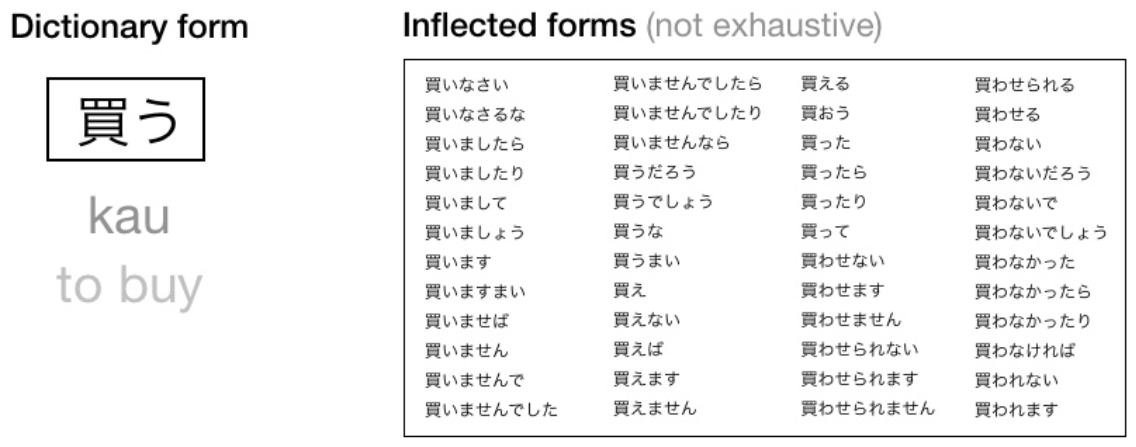
\includegraphics[width=0.7\textwidth]{image7.png}
    \caption{Example of the Japanese Base Form Filter in action.}
    \label{fig:base_form_filter}
\end{figure}

\subsubsection{Japanese Non-meaningful Terms Removal Filter}
\textit{JapanesePartOfSpeechStopFilterFactory} removes tokens with certain part-of-speech tags. For example, the particle “を” (wo), which marks the direct object of a verb, is removed from the token stream.

\subsubsection{Japanese Katakana Stemming}
\textit{JapaneseKatakanaStemFilter} normalizes common katakana spelling variations ending in a long sound character (ー) by removing it. Only katakana words longer than four characters are processed. For example, パーティー (pātī, "party") becomes パーティ (pāti), but コピー ("copy") remains unchanged as it is too short.

\section{Apache Solr Processing Flow Diagrams}

\begin{figure}[h!]
    \centering
    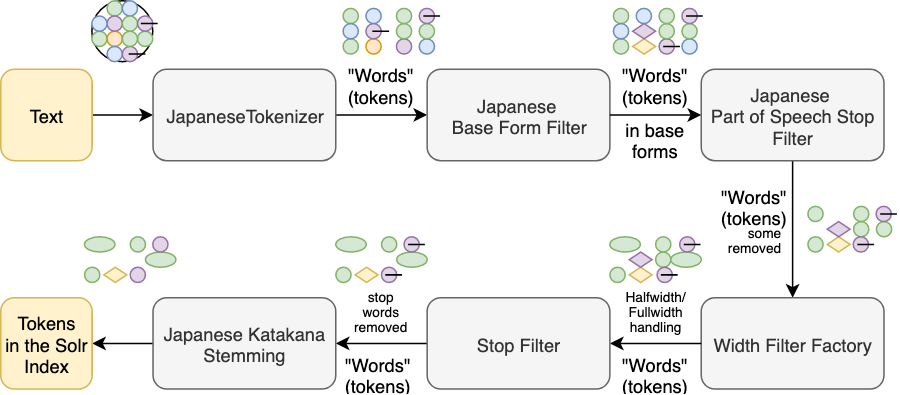
\includegraphics[width=0.9\textwidth]{schem1.png}
    \caption{Apache Solr processing flow for Japanese.}
    \label{fig:solr_japanese_flow}
\end{figure}

\begin{figure}[h!]
    \centering
    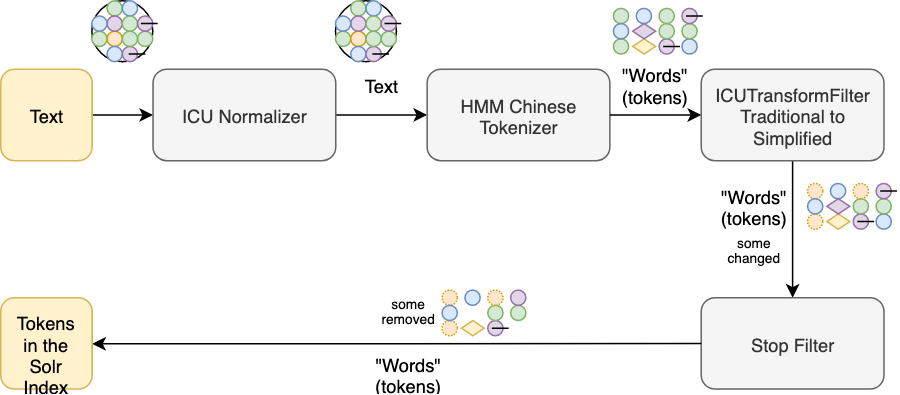
\includegraphics[width=0.9\textwidth]{chinese-japanese.png}
    \caption{Apache Solr Processing Flow for Chinese.}
    \label{fig:solr_chinese_flow}
\end{figure}

% --- NUMERALS ---
\section{Numerals}
In Japan and China, most people and institutions primarily use Arabic numerals. However, Chinese and Japanese numerals are also used, and the system must support them. Japanese numerals are often written using a combination of kanji and Arabic numbers with various kinds of punctuation. For example, 3.2千 means 3200.

Apache Solr comes with the \textit{JapaneseNumberFilter}, which normalizes various Japanese number formats to regular Arabic decimal numbers. This allows a search for "3200" to match "3.2千" in the text.

\begin{table}[h!]
    \centering
    \caption{Examples of Japanese Number Normalization via JapaneseNumberFilter.}
    \begin{tabular}{p{0.25\linewidth} p{0.15\linewidth} p{0.5\linewidth}}
    \toprule
    \textbf{Before} & \textbf{After} & \textbf{Comments} \\
    \midrule
    〇〇七 & 7 & 〇 (maru) is the same as numeral 0. \\
    三千2百2十三 & 3223 & \\
    3.2千 & 3200 & 千 means 1000. “.” is a double-byte point. \\
    4,647.100 & 4647.1 & Commas are ignored (removed). \\
    2,500万 & 25000000 & 万 means 10,000. \\
    \bottomrule
    \end{tabular}
    \label{tab:number_normalization}
\end{table}

This filter may in some cases normalize tokens that are not numbers. For example, 田中京一 is a name, but out of context 京一 can also represent a large number. Formal numbers (daiji) and decimal fractions are currently not supported by the filter.

% --- SYNONYMS and HOMOPHONES ---
\section{Synonyms and Homophones}
\subsection{Synonyms}
Like other languages, Japanese has multiple words for the same concept. For example, there are many verbs meaning "to kill": 殺す, 殺害する, 暗殺する, etc. Apache Solr supports synonyms, but the dictionary of synonymous words must be user-defined.

\subsection{Homophones}
Homophones are words that are pronounced the same but differ in writing and meaning. Because of a smaller stock of phonemes in Japanese and Chinese, the number of homophones is very large. For many homophones, a universally-accepted orthography does not exist, and the choice of character is often governed by the personal preferences of the writer. A semantically classified database of homophones is needed to implement effective cross-homophone searching. The table below shows the many ways to write the verb \textit{sasu}, depending on meaning.

\begin{table}[h!]
    \centering
    \caption{Orthographic Variants for the Japanese verb \textit{sasu}.}
    \begin{tabular}{llll}
    \toprule
    \textbf{English} & \textbf{Standard} & \textbf{Sometimes} & \textbf{Often also} \\
    \midrule
    to offer & 差す & さす & \\
    to hold up & 差す & さす & \\
    to pour into & 差す & 注す & さす \\
    to color & 差す & 注す & さす \\
    to shine on & 差す & 射す & さす \\
    to aim at & 指す & 差す & \\
    to point to & 指す & さす & \\
    to stab & 刺す & さす & \\
    to leave unfinished & さす & 止す & \\
    \bottomrule
    \end{tabular}
\end{table}

% --- SEARCH BY PRONUNCIATION ---
\section{Search by Pronunciation}
In Japanese, the pronunciation is directly mapped to the written words. Users often type words in hiragana (phonetic script) and then convert them to kanji or katakana. A robust search system should be able to handle queries typed phonetically. For example, a search for “とうきょうえ” (tōkyōe) should suggest or match “東京駅” (tōkyōeki, Tokyo Station), as their pronunciations are nearly identical.

\begin{figure}[h!]
    \centering
    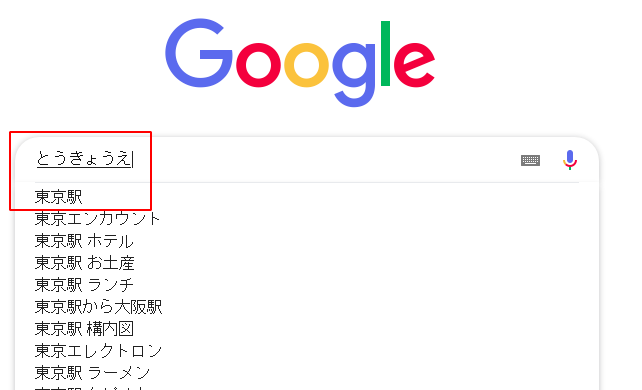
\includegraphics[width=0.7\textwidth]{image8.png}
    \caption{Google Suggest handling a phonetic Japanese query.}
    \label{fig:google_suggest_pronunciation}
\end{figure}

\begin{figure}[h!]
    \centering
    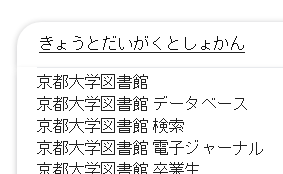
\includegraphics[width=0.7\textwidth]{image9.png}
    \caption{Search results for Kyoto University Library, likely initiated by a phonetic search.}
    \label{fig:kyoto_library_search}
\end{figure}

% --- PUNCTUATION ---
\section{Punctuation Marks}
There are punctuation marks specific for Japanese and Chinese, some of which have similar-looking but non-interchangeable equivalents in European languages.

\begin{table}[h!]
    \centering
    \caption{Specific CJK Punctuation Marks.}
    \begin{tabular}{c c p{0.5\linewidth}}
        \toprule
        \textbf{Mark} & \textbf{Example} & \textbf{Explanation} \\
        \midrule
        〜 & 1〜2 & Wavy dash, used for ranges. \\
        。 & & Full stop (equivalent to "."). \\
        、 & a、b、c & Enumeration comma. \\
        「 」 & 「あいうえお」 & Japanese equivalent of quotation marks. \\
        ・ & ジョン・ドゥ & Nakaten, used to separate parts of foreign names. \\
        \bottomrule
    \end{tabular}
\end{table}

% --- SEARCH UI OBSERVATIONS ---
\section{Search UI Observations}
Chinese and Japanese websites often have much less negative space, smaller images, and a higher density of information compared to Western sites. This layout style may be connected to a tendency for content efficiency, placing a maximum amount of content within a minimum space.

\subsection{Input Methods}
\subsubsection{Chinese Input}
Chinese text can be input in various ways, including Pinyin (Latin transcription), Wubi (stroke-based), handwriting, and voice recognition. Each method has its own user base and trade-offs.
\begin{itemize}
    \item \textbf{Wubi} is the fastest but most challenging method, requiring memorization of a stroke-to-key mapping.
    \item \textbf{Pinyin} is slower due to the need to select from a list of homonyms, but is common among the younger generation and foreigners.
    \item \textbf{Handwriting} and \textbf{Stroke sequence} are used by those who don't know Latin alphabets.
    \item \textbf{Image recognition} is great for larger amounts of data.
    \item \textbf{Voice recognition} is popular but challenged by the numerous dialects.
\end{itemize}

\begin{figure}[h!]
    \centering
    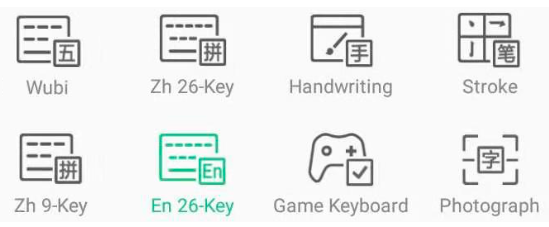
\includegraphics[width=0.8\textwidth]{Screen-Shot-2019-08-19-at-7.54.54-AM.png}
    \caption{Chinese input methods available on a standard Android system.}
    \label{fig:chinese_input_methods}
\end{figure}

\subsubsection{Japanese Input}
The primary input method is typing words by their reading in kana (phonetically) and then converting them to kanji. Because of many homonyms, a pop-up window often appears with a list of conversion variants. Japanese keyboards have special helper keys for conversion (変換), no conversion (無変換), and switching between kana modes.

\begin{figure}[h!]
    \centering
    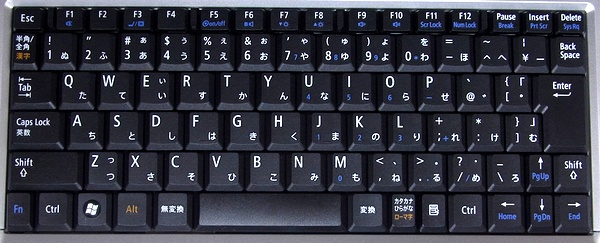
\includegraphics[width=0.8\textwidth]{image10.png}
    \caption{A typical Japanese keyboard layout.}
    \label{fig:japanese_keyboard}
\end{figure}

\subsection{Less Search, More Navigation}
It is common for Chinese and Japanese websites to de-emphasize the search field and prioritize navigation. With complex input methods, it is often faster for users to click through categories than to type a search query. Many apps use a "focus page" that appears when the search bar is clicked, offering tags and popular searches to guide the user and reduce the need for manual text entry.

\begin{figure}[h!]
    \centering
    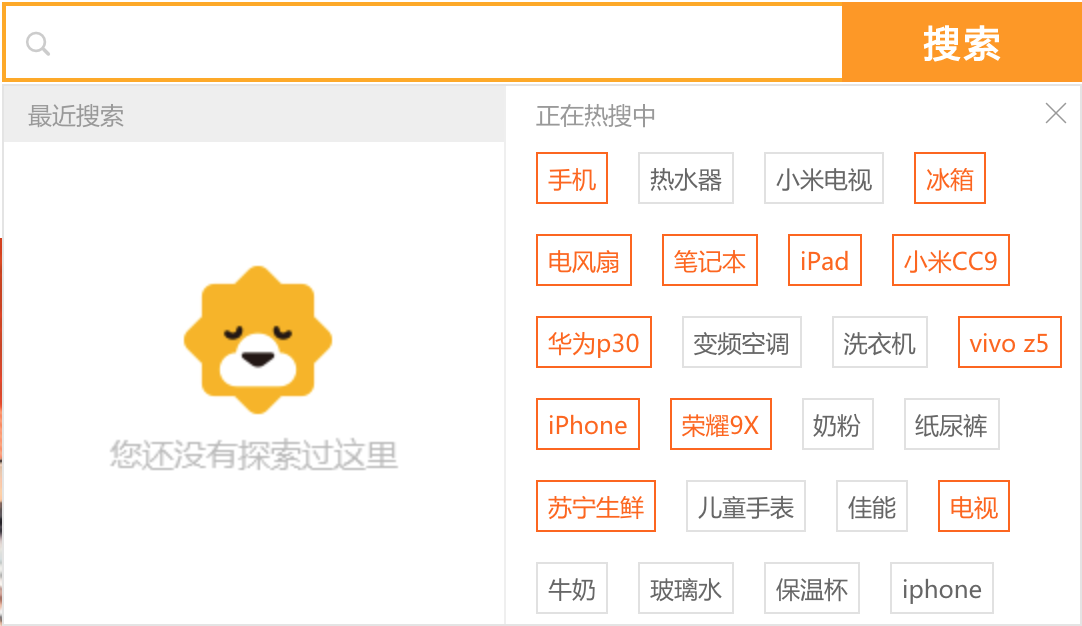
\includegraphics[width=0.8\textwidth]{image15.png}
    \caption{The search UI on Suning.com, showing popular search tags below the search bar.}
    \label{fig:suning_ui}
\end{figure}

\subsection{Other UI Trends}
\begin{itemize}
    \item \textbf{Voice Search:} Voice input for search queries is becoming increasingly common, especially for older audiences who may struggle with typing complex characters.
    \item \textbf{Context-aware Recommendations:} Many websites show recommended queries under the search bar that are based on user behavior and context.
    \item \textbf{Visual Search:} A growing number of e-commerce sites are implementing visual search, allowing users to find products by uploading an image.
    \item \textbf{Facets:} Facet panels are often arranged horizontally on Chinese websites due to the density of the script, while vertical facets remain more common on Japanese sites. All important facets are often expanded by default.
\end{itemize}

% --- RECOMMENDATIONS ---
\section{Recommendations}
\subsection{Implementation Questions}
If your website is available in different language versions, you need to have answers to the following questions:
\begin{itemize}
    \item What languages can be used on what language versions? Can I search in Chinese on the English website and vice versa?.
    \item Can we mix English and Chinese in the same query? This is especially important for brands and proper names (e.g., Sony / ソニー).
    \item What language variants (e.g., Simplified/Traditional Chinese) are supported?.
\end{itemize}

\subsection{Web Typography}
\begin{itemize}
    \item \textbf{Line Length:} The optimal line length is 15-40 characters for desktop and 15-21 for mobile, about half that recommended for English.
    \item \textbf{Fonts:} Use standard classifications like Mincho (serif) and Gothic (sans-serif) for Japanese, and Song/Ming (serif) and Hei (sans-serif) for Chinese. Avoid embedding large custom font files, as the large character sets can significantly slow page loading.
    \item \textbf{Styling:} Do not use italics, as it skews characters and makes them unreadable.
    \item \textbf{Font Size:} Use a minimum font size of 12pt, and consider 16pt for websites targeting older users. It's best to set font size with relative units like "em" or "\%" to respect user preferences.
\end{itemize}

% --- CONCLUSIONS ---
\section{Conclusions}
The challenges of Japanese and Chinese searching are significant but addressable. Because of the complexities and irregularities of their writing systems, successful implementation requires not only computational linguistic tools like morphological analyzers but also rich lexical databases fine-tuned to specific project goals and content. Both analyzers and databases are constantly improving, and it is important to keep an eye on the latest breakthroughs in information retrieval to continue delivering a better user experience.

\end{document}